\chapter{プロキシ}
プロキシ、根とスラングで言うところの串、これについてどんなイメージを持っているでしょうか。
まずは、プロキシがなんなのか、それを説明しましょう。

\section{いつものように昔話から始めよう}
さて、今は昔、20世紀に遡る。もしかしてIPアドレスが足りなくなっているんじゃないかということが判ってきた頃、IPv6がまだIPngという名前で呼ばれていた頃の話だ。

1996年2月にRFC1918として、プライベートIPアドレス割り当てが決定された。この時から、インターネットに直接接続されるグローバルアドレスと、インターネットに直接接続してはならないプライベートアドレスという区別ができた。それは、インターネットにアクセスできるホストと、インターネットにアクセスできないより多くのホスト、という区別卯もできたということでもある。

だが、インターネットに直接できないホストだからといって、インターネットにアクセスしなくていいわけではない。当時だと、メール、そして黎明期のWeb利用のため、インターネットの向こうにあるサーバにアクセスしたいというニーズがあった。\footnote{当時はコンテンツという洒落た言い方はまだ無かった。}

1996年5月にHTTP 1.0がRFC1945として纏められた。HTTPはそれ以前から存在していたが、RFCとして纏められたのはこのときである。この中には、プロキシについての記述がある。\footnote{RFC1945と、それ以降のHTTP1.1のRFCでは、プロキシ、ゲートウェイ、トンネルという三種の中継方法が定義されている。}このとき、プライベートネットワークからアクセスする手段として、プロキシがあったわけである。

では、Webを例にして、プロキシの動作を見て行くことにしよう。

\section{プライベートネットワークからのアクセス}
プライベートネットワークからアクスできるホストhの条件はなんであろうか。それは、プライベートなネットワークから到達できるホストである。NATがRFC2663として纏められるのは1999年まで待たなければならない。ここでは、NATがない時代の話をしていきたい。

余談ながらこの時代はまだルータというインターネットプロトコル層で中継を行う専用コンピュータにとっても黎明期であり、
余剰となったワークステーションがルータの役目を果たすことも多かった。

\subsection{それでもインターネットにアクセスしたい}

\begin{figure}[htbp]
	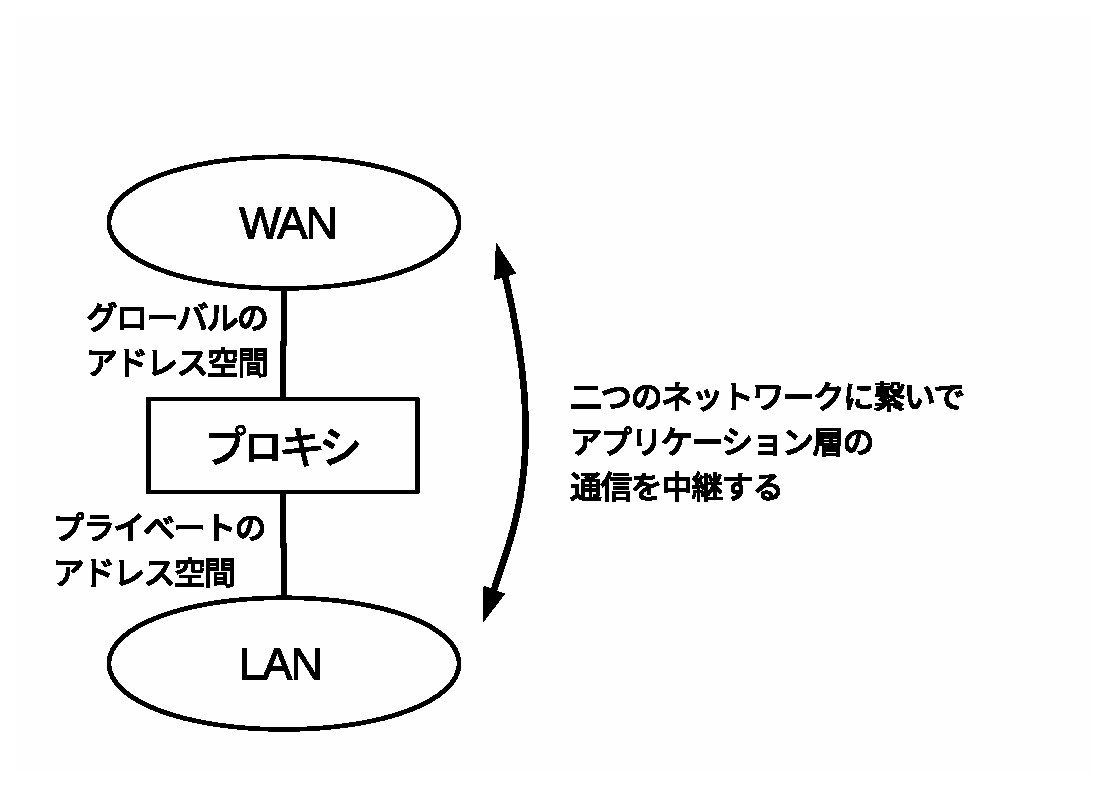
\includegraphics[width=12cm,clip]{draw/fig1.eps}
	\caption{プロキシの概念}
	\label{fig:proxy1}
\end{figure}

プライベートなアドレスを持つホストがアクセスできるのは、プライベートなアドレスを持つホストである。では、その条件でインターネットの向こうにあるサーバにアクセスするとしたらどうすれば良いだろうか。

それは、プライベートなアドレスのネットワークと、グローバルなアドレスのネットワークの両方に接続されているホストを用意して、そのホストにアクセスを中継してもらうことであるl。
HTTPのようなクライアント・サーバ型のアプリケーション層プロトコルであれば、リクエストをインターネットに中継し、レスポンスをプライベートなネットワークに中継するような機能を持つホストが入れがいいことになる。


当時、この役目を受け持つホストは、ネットワークの中で、ごく一部であった。つまり、プライベートのネットワークで共有するリソースであったわけだ。そうなる理由は簡単で、当時はネットワークインタフェイスの値段が高価だったためである。

本省では、このように、複数のネットワークに接続され、アプリケーション層の中継を行うホストを、プロキシと総称することにしよう。

\subsection{プロキシとルータの違い}

\begin{figure}[htbp]
	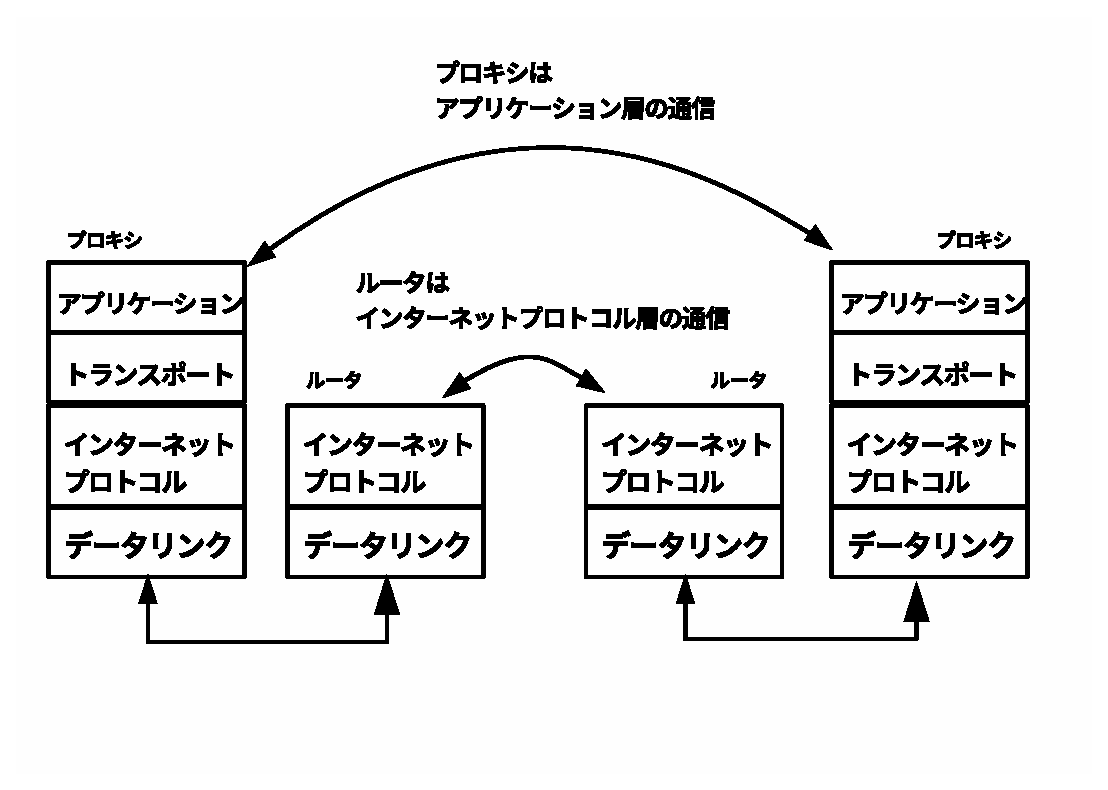
\includegraphics[width=12cm,clip]{draw/fig2.eps}
	\caption{プロキシとルータの違い}
	\label{fig:proxy and router}
\end{figure}

複数のネットワークにアクセスし、アプリケーション層の通信を中継するものをプロキシとy呼ぶ。ネットで中継を行う機器と言えば、ルータである。では、このルータとプロキシを比べてみよう。

結論からいけば、インターネットプロトコルスイートにおける、通信するレイヤーが異なる。

ルータは、インターネットプロトコル層の機能で、IPパケットを中継する。このとき、パケットはルーティングテーブルによって決定される宛先に転送される。ヘッダもペイロードも変更されない\footnote{正確には、転送後とにTTLが減少する。}

一方プロキシは、アプリケケーション層の中継である。アプリケーションが受信したリクエストやレスポンスを、アプリケーション層のプロトコルで送出する。このとき、プロトコルのコマンド、通信されるデータ、ともに非梅雨オナ変更が行われることがある。

\section{プロキシのかたち}
では、プロキシはどんな形で通信を中継するのだろう羽化。その分類に、RFC1945の分類を用いて、分類してみることにしよう。RFC1945では、プロキシ、ゲートウェイ、トンネルという分類がされている。

\subsection{プロキシ}

\begin{figure}[htbp]
	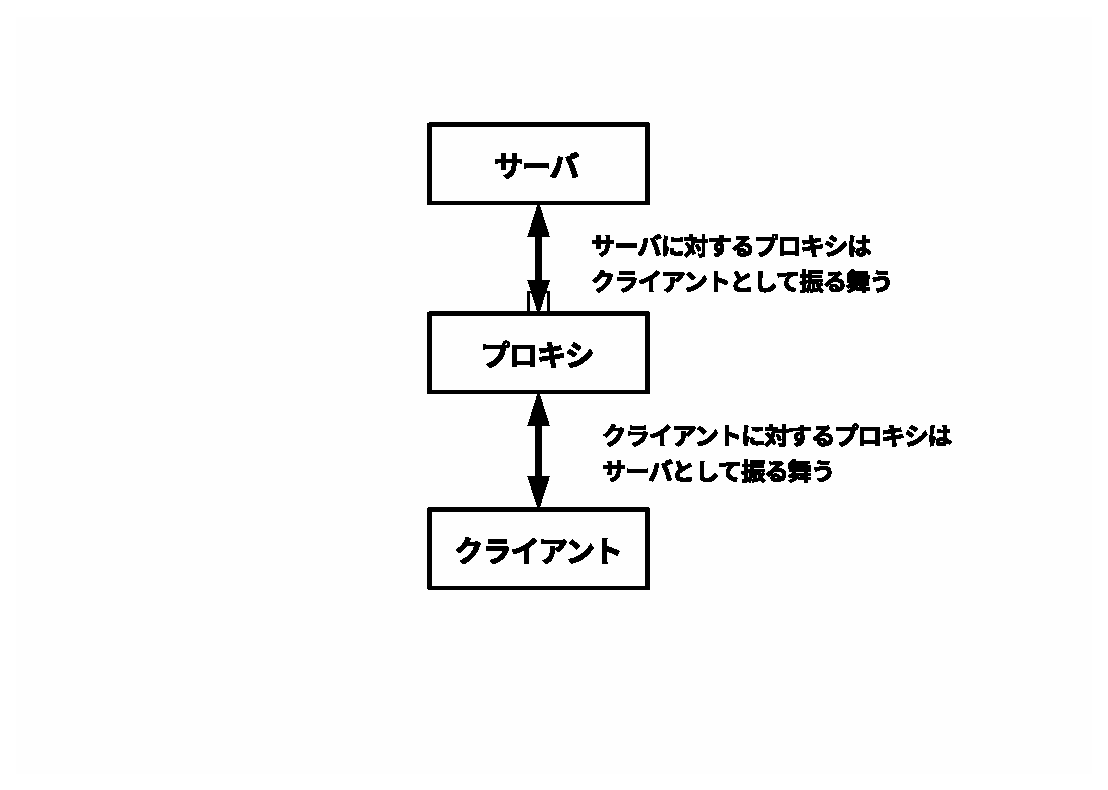
\includegraphics[width=12cm,clip]{draw/fig3.eps}
	\caption{プロキシ}
	\label{fig:proxy}
\end{figure}

通信をフォワーディングするものを、RFC1945ではプロキシとして定義している。ここでいうフォワーディングとは、どんな動作なのだろうか。

クライアントから、本来サーバに送られるリクエストを受け取る。そして、そのリクエストを、内容は変えず、自分自身がクライアントとなって発信する。
逆に、サーバからのレスポンスは、自分がクライアントとなって受信する。そのあとで、クライアントからのリクエストに対するレスポンスとして送出する。

つまり、プロキシは、本来のクライアントから見れば、サーバとしてふるまい、本来のサーバから見れば、プロキシはクライアントとして振る舞う。
そのため、HTTPのRFCでは、プロキシはクライアントとサーバの要件を共に満たさなければならないという要件が明記されている。

また、実際にクライアントがプロキシを利用するときは、どのプロキシサーバを利用するかという設定を明示的に行う必要がある。

ここまではHTTPで説明したが、SMTPについても同様に考えることが出来る。SMTPではプロキシという用語は使わず、メールのリレーという言い方をする。
内部から外へのメール転送はかならずこのサーバに転送する、というような指定をするわけだ。この場合、SMTPの仕様から、内部サーバもリレーホストのクライアントになる場合があることに注意したい。

\subsection{ゲートウェイ}

\begin{figure}[htbp]
	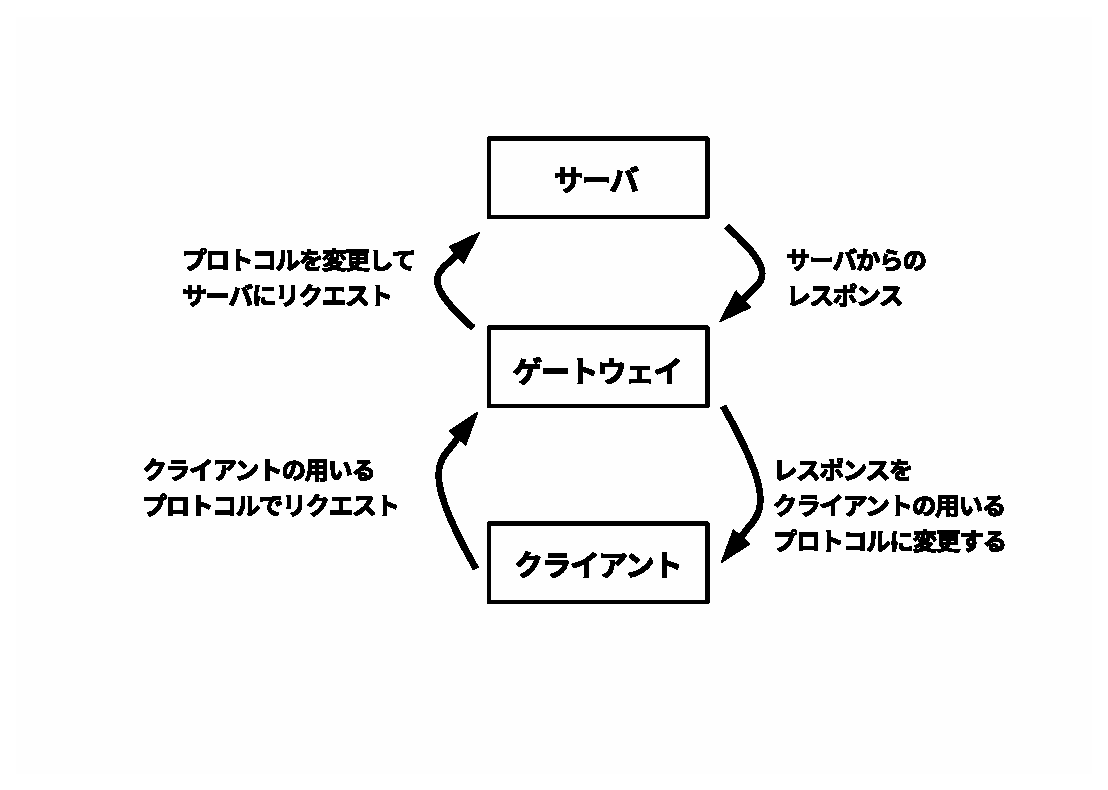
\includegraphics[width=12cm,clip]{draw/fig4.eps}
	\caption{ゲートウェイ}
	\label{fig:gateway}
\end{figure}

ゲートウェイは、プロトコルを変換するプロキシである。例えば、クライアントからの通信がHTTPであるとき、サーバにHTTPSでリクエストを出すプロキシは、ゲートウェイとなる。\footnote{TLS/SSLはセッション層のプロトコルとされることもあるが、ここではインターネットプロトコルスィートをモデルとしてアプリケーション層として扱う}

また、HTTPを利用してプロセス間通信を行うSOAPなどのプロトコルを、別のプロセス間通信のプロトコルに変換するプロキシも、ゲートウェイに該当する。

ゲートウェイはプロキシとして実装される場合と、次に説明するトンネルとして実装される場合とがアル。

\subsection{トンネル}

\begin{figure}[htbp]
	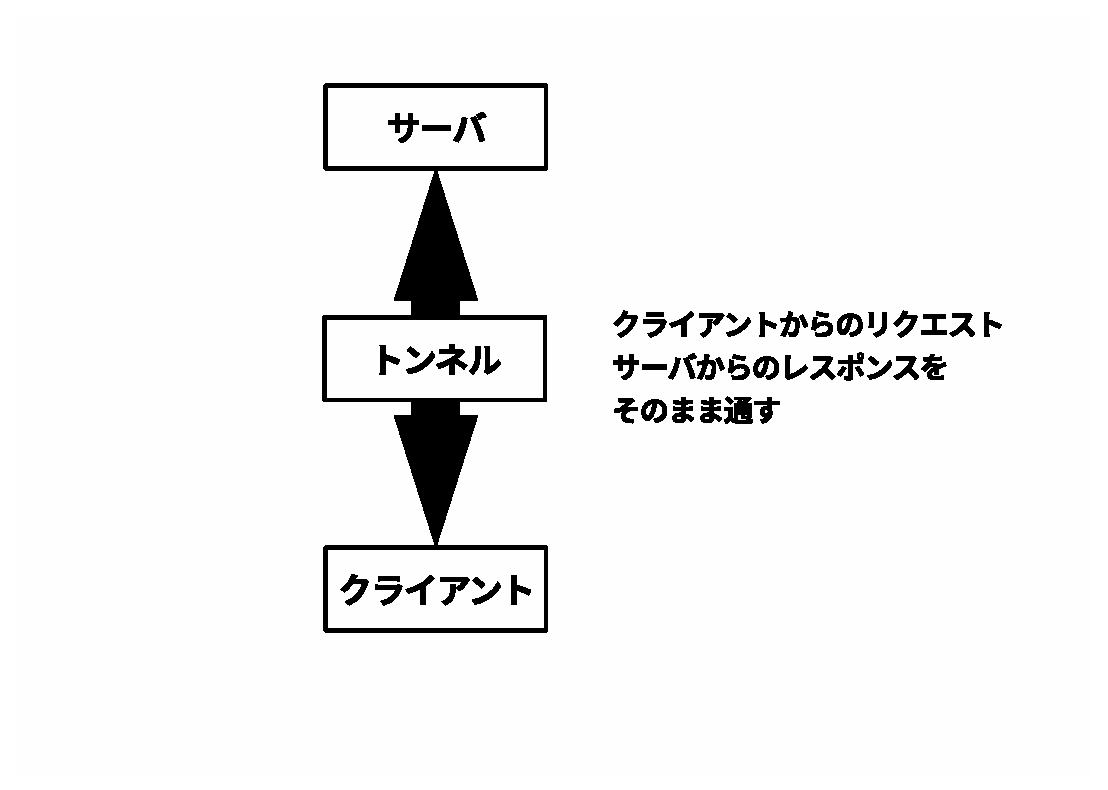
\includegraphics[width=12cm,clip]{draw/fig5.eps}
	\caption{トンネル}
	\label{fig:tunnel}
\end{figure}


トンネルは、クライアントから送信されたリクエストをそのままサーバに送出し、そのレスポンスも、そのままクライアントに返す。
そのため、トンネルは、クライアントとサーバが何らかの形で直接通信できる状況で用いられる必要がある。これについては、透過プロキシで説明することにしよう。

\subsubsection{透過プロキシ}
プロキシには、透過プロキシと呼ばれるものがある。トンネルに用いられる概念であるので、ここで説明しよう。

透過プロキシは、ネットワークのゲートウェイの手前に置かれる。
ここでいうゲートウェイは、アプリケ-ションのゲートウェイでなく、インターネットプロトコルのゲートウェイである。

このホストは、クライアントから外向けの通信が全て届く。そのなかで、たとえばSMTPやHTTPのリクエストを宛先にかかわらず内部に転送し、そのまま送り出す。サーバからのレスポンスについても同様である。

これは、クライアントから見ると、プロキシの存在を意識させない、つまりプロキシの設定が不要という利点がある。また、その性質から、ファイアウォールやUTMの機能として実装されることが多い。

トンネルとなるホストの内部処理で、宛先を見てリクエストやレスポンスを通すか通さないかという処理を行えば、それはファイアウォールの動作となる。

\section{プロキシの性質}
ここまでの説明である程度推測ができるのだが、アプリケーション層のプロキシには、いくつかの特徴的な性質がある。その性質について説明を行なおう。

それは、プロキシを介した通信のイニシエイターになれるのは、クライアント・サーバ型通信のクライアントだけであること、そして、プロキシが対応している特定のアプリケーションサービスしか利用できないことである。

また、プロキシは、複数のクライアントからの通信を同時に中継することができる。これは、クライアントからのリクエストを記録しておき、戻ってきたレスポンスを、リクエストを出したクライアントに返すことで実現される。

\subsection{どっち向きの通信?}
プロキシは、クライアント・サーバ型通信に対応した者となる。つまり、プロキシに接続された二つのネットワークのどちらから通信が始まるか、それが決まっているということだ。

一般に、LANなど内部がクライアント側、つまり通信のイニシエイターとなる。そして、外部は、その通信にたいする応答でのみ、通信をすることができる。ここでは、プロキシには方向があると言うことで捉えていてほしい。

\subsection{どの通信?}
プロキシは、アプリーション層の実装である。そのため、アプリケーション層のサービス毎tに、実装が必要となる。つまり、全ての通信を中継することが可能なプロキシは、現実的には存在しない、ということでもある。


\section{プロキシの役目}

さて、ここまでプロキシは、インターネットに直接接続できないネットワークとから、インターネットの特定のサービスにアクセスするための中継役という説明を行ってきた。だが、時代が下ると、プロキシにはそれ以外の役割が付与されるようになってきた。今度はそれについて説明をしよう。

\subsection{キャッシュ}
プロキシはリクエストとレスポンスを中継する。クライアントから見ればサーバであり、サーバから見ればクライアントであるのは、ここまで何度も説明したとおりだ。

サーバからのレスポンスは、同じデータが何度も届くことがある。例えば、サイトのロゴの画像など、同じデータが何度もレスポンスされる典型だろう。
このデータをプロキシが蓄積する。同じデータへのリクエストであれば、サーバにリクエストを出さず、プロキシが蓄積したデータを、レスポンスとしてクライアントに返す。これが、データを蓄積してサーバに変わって応答するキャッシュである。

こうすることで、インターネット経由でのサーバアクセスを減らすことができる。そして、実際のサーバへのリクエストを経ずにレスポンスが戻るので、クライアントから見た応答時間が早くなる。かつて、インターネット回線へのアクセスが遅く、高価であった時代には、重要なことであった。

そのデータをキャッシュすることを許可するか、許可するならどのくらいの時間の生存を赦すかは、レスポンスとしてデータを送り出すサーバ側の設定で決める。

\subsection{セキュリティ}
プロキシには、副次的な側面としてセキュリティのために用いられることがあるl。

ひとつは、特定のユーザのみプロキシを経由してノサーバアクセスを許可する場合。これは、プロキシ接続時に、何らかの形で認証を行う。こうすることで、許可されたクライアントのみが、プロキシを経由してサービスにアクセスすることが出来る環境を作ることが出来る。

また、プロキシは、必ず、クライアントからのリクエストと、サーバからのレスポンスを受け取る。そこで、そのリクエストやレスポンスを検査することで、事前登録された危険なサイトへのアクセスを防止し、ウィルスの付いたデータを受け取ることを抑止することが出来る。

\section{リバースプロキシ}

\begin{figure}[htbp]
	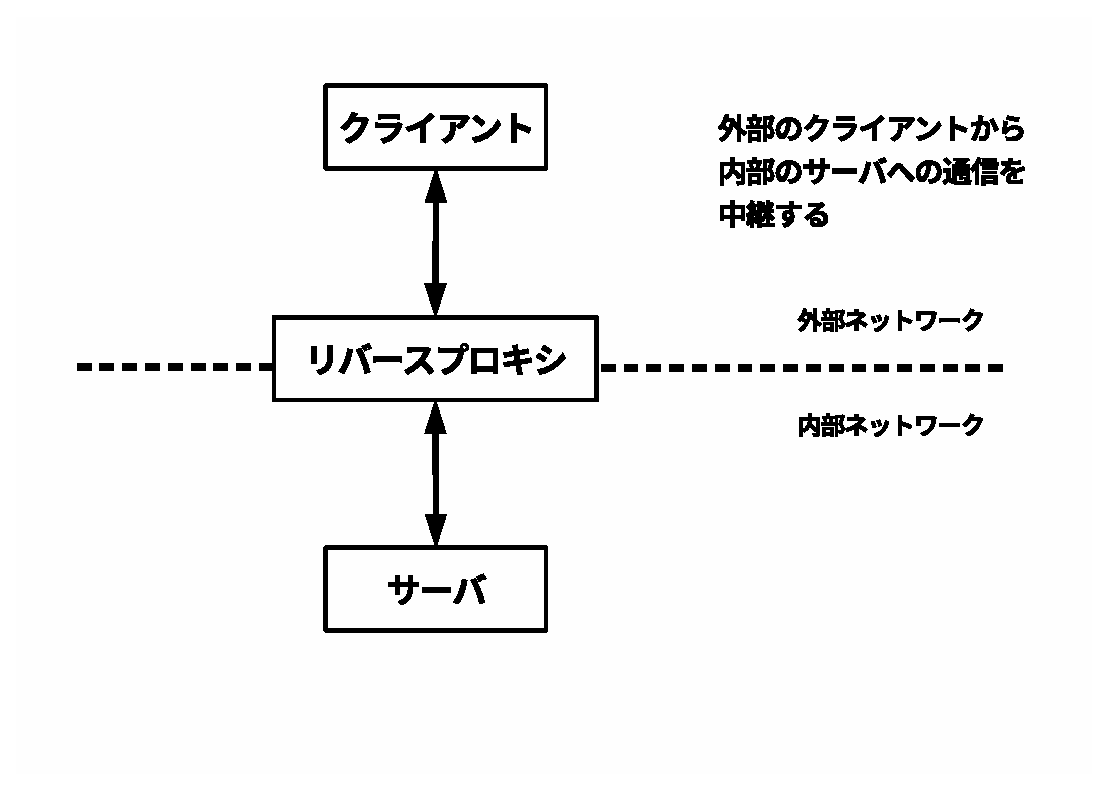
\includegraphics[width=12cm,clip]{draw/fig6.eps}
	\caption{リバースプロキシ}
	\label{fig:reverse-proxy}
\end{figure}

ここまでは、LANの中からインターネットへアクセスするという前提で、プロキシについて説明を行った。では、プロキシのクライアントとサーバの場所を逆にしたらどうなるであろうか。

インターネット経由でアクセスしてくるクライアントに、プロキシ経由でLAN内のサーバにアクセスするという構図になる。このプロキシで認証や、SSLによる暗号化を行う\footnote{このような用途で使うプロキシを、SSL-VPN送致と呼ぶ}ことで、安全にLAN内のサーバにアクセスさせることができる。

このような用途で使うプロキシを、通常とは逆向きに、外部がクライアント、内部がサーバとなるように設置される。つまり、通常とは逆、という意味で、リバースプロキシと呼んでいる。

\subsection{ロードバランサというプロキシ}
最後に、リバースプロキシの応用として、ロードバランサについて説明しよう。

サービスを行うサーバの負荷分散方法として、同じサーバを複数並べ、併用するという方法がある。だが、この方法の問題は、クライアントがどのサー^場にアクセスするのかを、何らかの方法で決定しなければならない9ということである。

ここで、リバースプロキシを使う。リバースプロキシがクライアントからアクセスを受け、複数あるサーバのいずれかに送出する。この時、サーバを選択する方法は、確率的に決める、サーバの負荷で決定する、などがある。このどれを使うかは、リバースプロキシの実装と設定次第だ。

また、サーバの死活監視も行い、生きているサーバにのみアクセスするようにすれば、クライアントから、サーバの停止が見えなくなるという利点もある。

リバースプロキシをこのような目的で使う場合、これはロードバランサと呼ばれる。

